\documentclass{article}
\usepackage[a4paper, total={5.5in, 8in}]{geometry}

\usepackage[T1]{fontenc}
\usepackage[french]{babel}
\usepackage[autolanguage]{numprint} % for the \nombre command
\usepackage{multicol}
\usepackage{wrapfig}

\usepackage{hyphenat, tikz, float, subcaption}
\hyphenation{mate-mática recu-perar}

\usepackage{graphicx}
\graphicspath{ {./images} }

\usepackage{caption}
\usepackage{subcaption}
\captionsetup{position=below}

\sloppy % pour pas que ça dépasse
\newtheorem{definition}{Définition}

\def\Cpp{C\texttt{++} }

\title{Rapport CGDI}
\author{Corto Cristofoli et Max Royer}


\begin{document}
\maketitle
% \tableofcontents



\section{Introduction}
Cet article est réalisé dans le cadre de notre cours de CGDI.
Il s'agit de la présentation de notre implémentation de l'article
de recherche \textit{Curved PN triangle}, par Alex Vlachos, Jorg Peters,
Chas Boyd et Jason L. Mitchell.

L'article présente un algorithme de lissage de modèles 3D de basse résolution.
Pour cela, l'idée est d'utiliser la méthode des « Curved PN triangles ». Un
modèle 3D de basse résolution n'a que peu de polygones et donc une alure
nécessairement anguleuse. Pour le rendre plus organique un lissage est
nécessaire : il faut rajouter un grand nombre de triangle afin de faire
disparaître ces angles. Ce rajout se fait algorithmiquement en suivant des
surfaces de Bézier triangulaires.

Si l'article décrit l'algorithme de manière théorique, nous nous sommes penchés
sur sa compréhension et son implémentation en \Cpp à l'aide de la
bibliothèque \textbf{geometry-central}.


\section{Principe de l'algorithme}

\begin{figure}[ht!]
\centering
    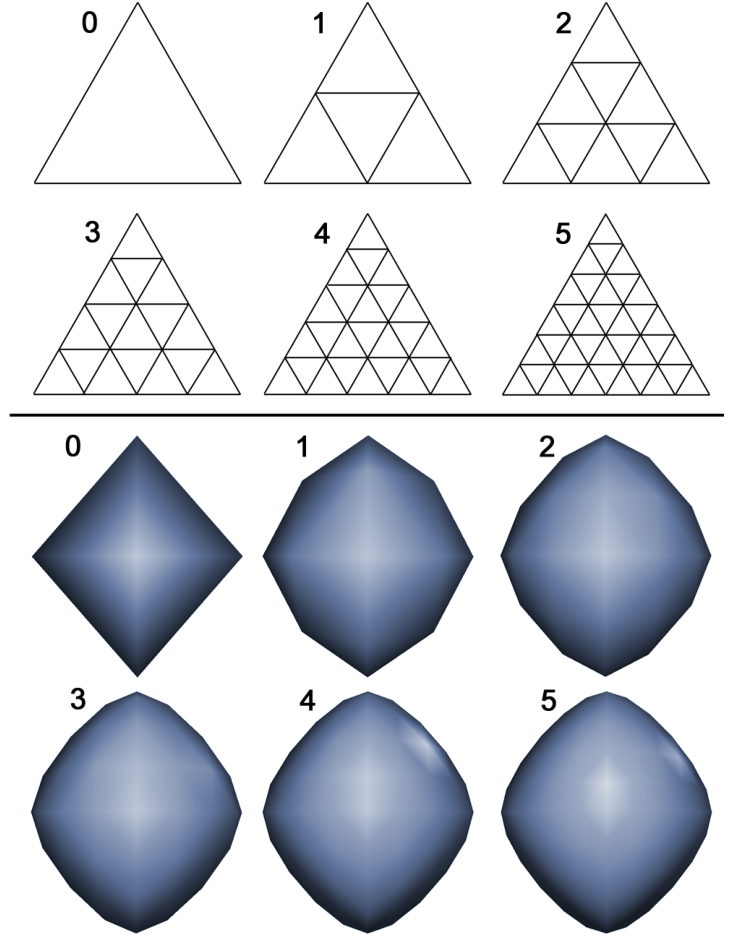
\includegraphics[width=0.4\linewidth]{lod}
    \caption{Sous-triangulation en fonction du \texttt{lod} (de 0 à 5)}
    \label{fig:lod}
\end{figure}

Dans tout le rapport nous considérons qu'un modèle 3D est un ensemble de face
triangulaires. Il est facile de se ramener à ce cas ci en triangulant
simplement les faces non triangulaires.

L'algorithme vise à transformer chaque faces triangulaires en une multitude,
dépendant d'un facteur : le \textit{level of detail} ou \texttt{lod}.

Concrètement, le \texttt{lod} correspond au nombre de sommets à ajouter sur une
arête du triangle d'origine (voir \ref{fig:lod}).

% TODO: expliquer pourquoi ce choix du nombre de points de contrôle
Une fois la subdivision faites pour chaque face (on verra plus tard que cette
subdivision pose des soucis d'implémentation), il faut moduler la position des
nouveaux sommets afin de parvenir à un lissage convainquant. Pour se faire, on
utilise une surface de Bézier triangulaire avec 10 points de contrôle. Les
différents sommets des nouvelles faces seront ensuite placés de manière à
suivre la surface de Bézier produite. Si l'on nomme $b_{ijk}$ avec $i+j+k = 3$
et $i,j,k\geq 0$, alors la position d'un des points du triangle aux coordonnées
barycentrique $(u,v)$ est définie dans l'espace par le patch de bézier $b$
($w=1-u-v$) : $$b(u,v) = \sum_{i+j+k=3} b_{ijk} \frac{3!}{i!j!k!}u^i v^i w^i$$

Voyons maintenant comment calculer les différents $b_{ijk}$.

\section{Calcul des points de contrôle du patch de Bézier}

\begin{figure}[ht!]
\centering
    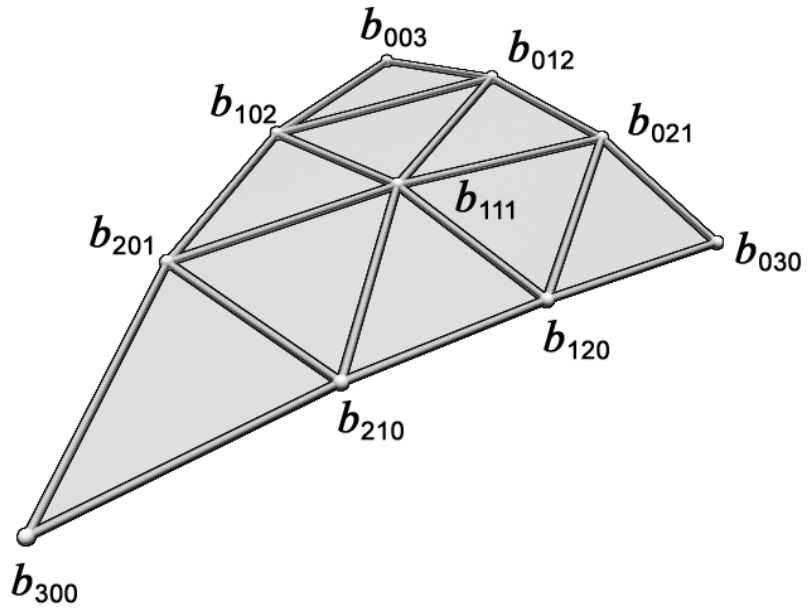
\includegraphics[width=0.4\linewidth]{control-points}
    \caption{Points/coefficients de contrôle d'un patch de Bézier triangulaire}
    \label{fig:control-points}
\end{figure}

En s'appuyant sur la figure \ref{fig:control-points}, on peut distinguer 3
catégories de coefficients:

\begin{itemize}
    \item \textit{coefficients de sommets} : $b_{300}, b_{030}, b_{003}$
    \item \textit{coefficients tangents} : $b_{210}, b_{201}, b_{120},
b_{021}, b_{102}, b_{012}$
    \item \textit{coefficient central} : $b_{111}$
\end{itemize}

\subsection{Coefficients de sommets}
Afin de conserver la forme primaire du modèle, les sommets originaux ne change
pas de position dans l'espace : la position des coefficients de sommets est
donc la même que celle de leur sommet respectif (si l'on applique $b$ à
$(1,0)$, $(0,1)$ ou $(0,0)$ on voit bien que les positions sont respectivement
$b_{300}$, $b_{030}$ ou $b_{003}$).

\subsection{Coefficients tangents}
Afin de calculer les coefficients tangents introduisons la notion de normale à
un point.

\begin{definition}{Vecteur normal à un point}

Les modèles 3D que nous étudions sont des modèles orientés, c'est-à-dire que
chaque face du modèle est définie par un unique vecteur unitaire, normal à la
surface et orienté vers l'extérieur du modèle.

Soit $s$ un sommet du modèle et $f_a,f_b,f_c$ les faces auxquelles il
appartient (si il y a un bord cela ne change pas grand chose). Le vecteur
normal au sommet $s$ est la moyenne des vecteurs normaux de chaques faces :
$N_s = \frac{N_a + N_b + N_c}{||N_a + N_b + N_c||}$.
\end{definition}

\begin{figure}[ht!]
\centering
    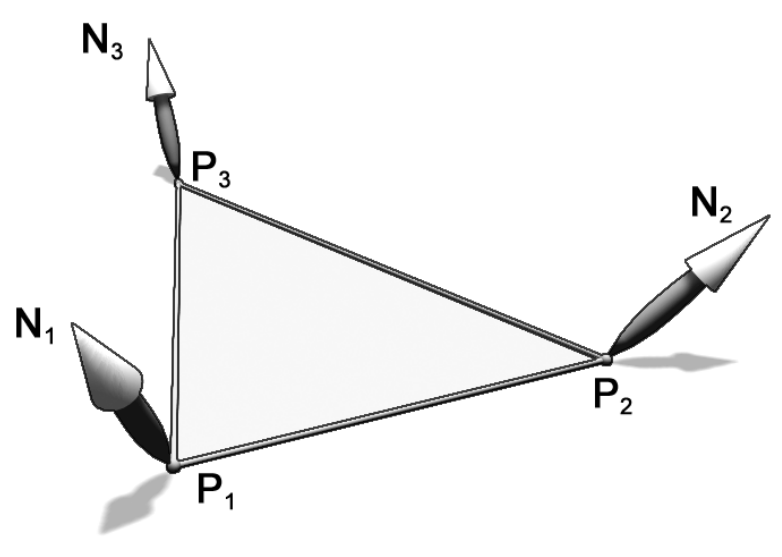
\includegraphics[width=0.4\linewidth]{normals}
    \caption{Données en entrée : points $P_i$ et leur normale $N_i$}
    \label{fig:normals}
\end{figure}

\begin{figure}[ht!]
\centering
    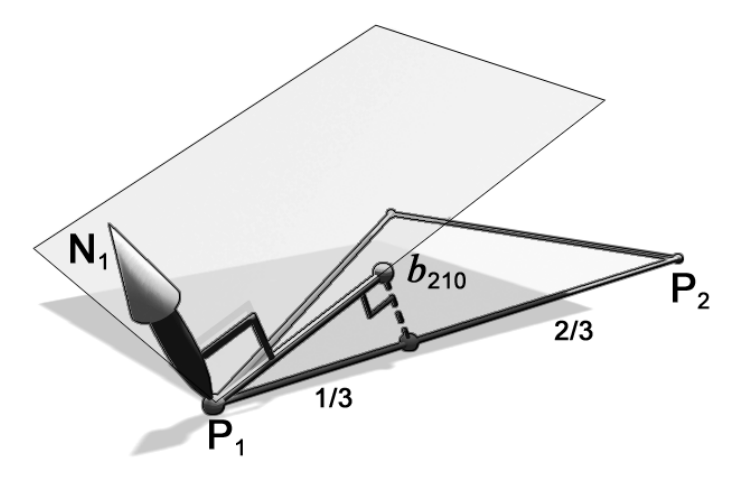
\includegraphics[width=0.4\linewidth]{tangent}
    \caption{Construction du coefficient tangent $b_210$ en projettant dans le
plan de $N_1$}
    \label{fig:tangent}
\end{figure}

Pour chaque sommets, le vecteur normal induit un plan normal. On choisit donc
de projeter chaque coefficient tangent dans le plan normal du sommet le plus
proche (voir figure \ref{fig:tangent})

\subsection{Coefficient central}

\section{Enjeux d'implémentation de \textit{Geometry Central}}
% Où on explique comment fonctionne `geometry-central` avec uniquement la
% possibilité d'ajouter des sommets à des faces (ou edges) ce qui fait
% trianguler automatiquement. D'où l'importance de repartir de zero.
% (je peux le faire ça)

\section{Indexation des sommets du modèle 3D}

\begin{figure}[H]
\centering
\begin{tikzpicture}
\draw (0,0)--(5.19,3) node[black,above]{\texttt{6}}node[gray,right]{$P_{1}$};
\draw (5.19,3)--(5.19,-3)node[black,below]{\texttt{9}}node[gray,right]{$P_{2}$};
\draw (5.19,-3)--(0,0)node[black,below]{\texttt{0}}node[gray,left]{$P_{0}$};
\draw (1.73,1)node[black,above]{\texttt{1}}--(1.73,-1)node[black,below]{\texttt{2}};
\draw (3.46,2)node[black,above]{\texttt{3}}--(3.46,0)node[black,right=0.17cm]{\texttt{4}};
\draw (3.46,0)--(3.46,-2)node[black,below]{\texttt{5}};
\draw (3.46,2)--(5.19,1)node[black,right]{\texttt{7}};
\draw (3.46,-2)--(5.19,-1)node[black,right]{\texttt{8}};
\draw (1.73,1)--(5.19,-1);
\draw (1.73,-1)--(5.19,1);
\draw[gray,dashed] (0,-0.5)--(0,-3.5)node[below]{Couche 0};
\draw[gray,dashed] (1.73,-1.5)--(1.73,-3.5)node[below]{Couche 1};
\draw[gray,dashed] (3.46,-2.5)--(3.46,-3.5)node[below]{Couche 2};
\draw[gray,dashed] (5.19,-3.5)--(5.19,-3.5)node[below]{Couche 3};
\end{tikzpicture}
\caption{Indexation de la triangulation d'une face pour un \texttt{lod} de 2}
\end{figure}

On numérote la discrétisation de la face de cette manière pour avoir facilement les nouvelles faces. En effet on remarque que pour un sommet $i$ dans une couche $c$, on a que ses deux voisins dans la couche $c+1$ sont les sommets $i+c+1$ et $i+c+2$. Cela permet de déduire rapidement les nouvelles faces à ajouter en disant que pour une discrétisation avec un \texttt{lod} $l$, on ajoute pour chaque sommets $i$ dans une couche $c$ avec $c\leq l$ la face $(i,i+c+1,i+c+2)$ et la face $(i,i+c+2,i+1)$ si $i+1$ est aussi dans la couche $c$ (\textit{i.e.} $i+1< \frac{(c+2)(c+1)}{2}$)
\begin{figure}[H]
\centering
\begin{tikzpicture}
    \draw (0,0)--(5.19,3)node[black,right]{\texttt{j+1}};
\draw (5.19,3)--(5.19,-3);
\draw (5.19,-3)--(0,0);
\draw[line width=0.35mm,red] (1.73,1)node[black,above]{\texttt{i}}--(1.73,-1)node[black,below]{\texttt{i+1}};
\draw[line width=0.35mm,red] (3.46,2)node[black,above left]{\texttt{i+c+1}}--(3.46,0)node[black,right=0.17cm]{\texttt{i+c+2}};
\draw[line width=0.35mm,red] (1.73,1)--(3.46,2);
\draw[line width=0.35mm,red] (1.73,1)--(3.46,0);
\draw[line width=0.35mm,red] (1.73,-1)--(3.46,0);
\draw (3.46,0)--(3.46,-2)node[black,below]{\texttt{j}};
\draw (3.46,2)--(5.19,1);
\draw (3.46,-2)--(5.19,-1);
\draw (3.46,0)--(5.19,-1);
\draw (3.46,0)--(5.19,1);
\draw[gray,dashed] (1.73,-1.5)--(1.73,-3.5)node[below]{Couche \texttt{c}};
\end{tikzpicture}
\caption{Exemple de faces ajoutées pour un sommet \texttt{i} dans la couche \texttt{c} ainsi que le cas où \texttt{j} et \texttt{j+1} ne sont pas dans la même couche}
\end{figure}

Chaque sommets est alors identifié par ses coordonnées barycentriques en fonction de $(P_{0},P_{1},P_{2})$, étant donné que ces coordonnées sont rationnelles et sont en fait des multiples de $\frac{1}{\texttt{lod}+1}$ nous avons décider de garder des coordonnées entières pour identifier les sommets tout en gardant le \texttt{lod} lorqu'il s'agit de calculer la position du sommet dans la tuile de Bézier.

Ainsi un sommet est représenté par un \texttt{vector} de \texttt{pair(int,int)} de taille 3, tel que pour chaque pair, le premier élément est l'indice du point $P_{i}$ et le second est la coordonnée barycentrique associée au point $P_{i}$.
\begin{figure}[H]
\centering
\begin{tikzpicture}
    \draw (0,0)node[black,left]{$P_{0}$}--(1.73,1);
\draw (0,0)--(1.73,-1);
\draw (1.73,-1)--(3.46,0)node[black,right]{$P_{3}$};
\draw (1.73,1)--(3.46,0);
\draw (1.73,1)node[black,above]{$P_{1}$}--(1.73,-1)node[black,below]{$P_{2}$};
\fill (1.73,0) circle (2pt) node[right] {$P$};
\end{tikzpicture}
\caption{Exemple de double représentation pour un seul et même point}
\label{fig:doublerepr}
\end{figure}

Ici le sommet $P$ peut être représenté par: $\left\{(P_{0},0),(P_{1},\frac{1}{2}),(P_{2},\frac{1}{2})\right\}$ mais aussi par $\left\{(P_{1},\frac{1}{2}),(P_{2},\frac{1}{2}),(P_{3},0)\right\}$. Au départ nous avons pensé naïvement à directement calculer la valeur du points dans la tuile de Bézier associé car lui pour le coup sera "le même" que pour les autres représentations. Malheureusement cette approche n'est pas concevable car les arrondis sur les \texttt{double} ne nous garantiraient pas que l'identification d'un point soit unique. Nous allons voir comment régler ce problème après avoir décris la classe \texttt{Obj}.

Pour recréer un nouvel objet nous avons créé une petite classe \texttt{Obj} ayant les primitives pour construire un tel objet. Le problème est qu'un point identique peut avoir plusieurs représentation possibles. Par exemple pour:

\begin{figure}[H]
\centering
\begin{tikzpicture}
\draw
    (0,0)  node[draw] (O) {\texttt{Obj}}
    (-4,3)  node {Fields}
    (-4,2)  node[gray,draw]                 (i) {\texttt{index\_vertices}}
    (-4,1)  node[gray,draw]                 (v) {\texttt{vertices}}
    (-4,0)  node[gray,draw]                 (f) {\texttt{faces}}
    (-4,-1)  node[gray,draw]                 (n) {\texttt{normals}}
    (-4,-2)  node[gray,draw]                 (nb) {\texttt{nb\_points}}
    (4,3)  node {Methods}
    (4,1.5)  node[gray,draw]                 (av) {\texttt{add\_vertex()}}
    (4,0.5)  node[gray,draw]                 (af) {\texttt{add\_face()}}
    (4,-0.5)  node[gray,draw]                 (gi) {\texttt{get\_index\_or\_assign()}}
    (4,-1.5)  node[gray,draw]                 (w) {\texttt{write\_to\_file()}};
\draw (O) -- (i);
\draw (O) -- (v);
\draw (O) -- (f);
\draw (O) -- (n);
\draw (O) -- (nb);
\draw (O) -- (av);
\draw (O) -- (af);
\draw (O) -- (gi);
\draw (O) -- (w);
\end{tikzpicture}
\caption{Description de la classe \texttt{Obj}}
\end{figure}

Ici on a \texttt{Obj.index\_vertices : map<vector<pair<int,int>>,int>}, cela veut dire que l'on doit être capable d'ordonner les représentations des points en coordonnées barycentrique tout en conservant leur équivalence.

Pour cela nous effectuons d'abord un tri sur le \texttt{vector} des coordonnées de manières à trier selon l'ordre lexicographique inversé sur l'ordre et sur les coordonnées, \textit{i.e.}:

\begin{equation}
(i,j) <_{pair} (k,l) \Leftrightarrow l < j \textrm{ ou } \left(l=j\textrm{ et } k < i\right)
\end{equation}


Cela permet alors d'ordonné facilement les représentations triées en considérant l'ordre lexicographique sur la partie ou la représentation a des coordonnées strictement positives. Pour exemple reprenons les deux représentations de la figure \ref{fig:doublerepr}.
\begin{figure}[H]
\centering
\begin{subfigure}{.49\textwidth}
    \centering
\scalebox{0.8}{
  \begin{tikzpicture}
    \draw (-3,0)node[draw]{$\left\{(\texttt{0},0),(\texttt{1},\frac{1}{2}),(\texttt{2},\frac{1}{2})\right\}$};
    \draw (3,0)node[draw]{$\left\{(\texttt{1},\frac{1}{2}),(\texttt{2},\frac{1}{2}),(\texttt{3},0))\right\}$};
    \draw[gray,dashed,->] (0,-0.5)--(0,-1.5)node[midway,right]{Tri};
    \draw (-3,-2)node[draw]{$\left\{(\texttt{2},\frac{1}{2}),(\texttt{1},\frac{1}{2}),(\texttt{0},0))\right\}$};
    \draw (3,-2)node[draw]{$\left\{(\texttt{2},\frac{1}{2}),(\texttt{1},\frac{1}{2}),(\texttt{3},0))\right\}$};
    \draw[gray,dashed,->] (0,-2.5)--(0,-3.5)node[midway,right]{Retrait des coodornées nulles};
    \draw (-3,-4)node[draw]{$\left\{(\texttt{2},\frac{1}{2}),(\texttt{1},\frac{1}{2}))\right\}$};
    \draw (3,-4)node[draw]{$\left\{(\texttt{2},\frac{1}{2}),(\texttt{1},\frac{1}{2}))\right\}$};
    \draw (0,-4)node {=};
\end{tikzpicture}}
\end{subfigure}
\begin{subfigure}{.49\textwidth}
    \centering
\scalebox{0.8}{
  \begin{tikzpicture}
    \draw (-3,0)node[draw]{$\left\{(\texttt{0},0),(\texttt{1},\frac{1}{2}),(\texttt{3},\frac{1}{2})\right\}$};
    \draw (3,0)node[draw]{$\left\{(\texttt{1},\frac{1}{2}),(\texttt{2},\frac{1}{2}),(\texttt{3},0))\right\}$};
    \draw[gray,dashed,->] (0,-0.5)--(0,-1.5)node[midway,right]{Tri};
    \draw (-3,-2)node[draw]{$\left\{(\texttt{3},\frac{1}{2}),(\texttt{1},\frac{1}{2}),(\texttt{0},0))\right\}$};
    \draw (3,-2)node[draw]{$\left\{(\texttt{2},\frac{1}{2}),(\texttt{1},\frac{1}{2}),(\texttt{3},0))\right\}$};
    \draw[gray,dashed,->] (0,-2.5)--(0,-3.5)node[midway,right]{Retrait des coodornées nulles};
    \draw (-3,-4)node[draw]{$\left\{(\texttt{3},\frac{1}{2}),(\texttt{1},\frac{1}{2}))\right\}$};
    \draw (3,-4)node[draw]{$\left\{(\texttt{2},\frac{1}{2}),(\texttt{1},\frac{1}{2}))\right\}$};
    \draw (0,-4)node {>};
    \draw (-5.3,0)--(-5.3,-4);
\end{tikzpicture}}
\end{subfigure}
\caption{Exemples d'ordres sur des représentations}
\end{figure}

Ainsi on peut passer à la \texttt{map} la structure de comparaison adéquate pour savoir si on a déjà ajouté le point dans \texttt{Obj.vertices}.
\end{document}
